\section{An End-to-End Multi-Task and Fusion CNN for Inertial-Based Gait Recognition}

\begin{flushleft}
    \author{
    Rubén Delgrado-Esca$ \tilde{n} $o,
    Francisco M. Castro,
    Julián Ramos Cózar,
    Manuel J. Marín-Jiménez,
    and Nicolás Guil
    }
\end{flushleft}

\begin{center}
    \emph{IEEE DIGITAL OBJECT IDENTIFIER}
\end{center}

\subsection{INTRODUCTION}
An individual's gait appears as their own fingerprint. The study of this 
topic doesn't not only concern the area of medicine, but also that of security 
and identification. The gating study is based on a non-invasive system that 
collects patterns without the direct intervention of the subject. The data, 
which allow the recognition of the gait, are taken by inertial sensors present 
in a multitude of devices such as smartphones or smartwatches. A system 
is presented that uses a convolutional neural network (CNN) that uses the 
data collected by these inertial sensors to be able to predict the subject. The 
approach followed is the one in figure \ref{fig:preview}. Two extensions have been added 
to the network. The first deals with merging sensory data, while the second 
deals with improving the learning process and producing multiple outputs 
from a single input, thanks to a multi-task scheme. The tasks considered 
are: identification, gender recognition and age estimation. The dataset used 
is OU-ISIR gait database \cite{0857651721}, containing information such as inertial sensors 
such as accelerometers and gyroscopes.
\begin{figure}[htbp]
    \centering
    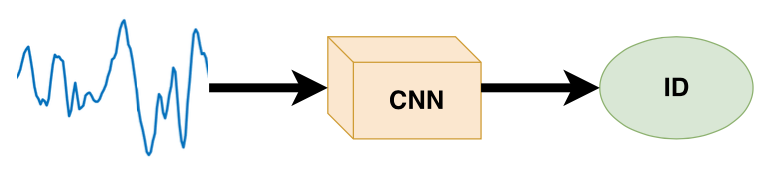
\includegraphics[width = 0.6 \linewidth]{images/paper5/usecase.png}
    \centering
    \caption{A preview of how the model works.}
    \label{fig:preview}
\end{figure}

\subsection{RELATED WORK}
Some methods have placed inertial sensors in different parts of the body 
such as legs \cite{0857651733}, hips \cite{0857651732}, ankles, or even in objects such as bags [35] and 
pockets \cite{0857651720}. Other methods \cite{0857651736} directly use all the inertial sensors present 
in the smartphone. With the advent of deep learning and CNNs, classifying 
an activity has turned out to be an easier job. The input provided to these 
networks is either the raw data of the inertial sensors, or the images that 
represented such data. The entire sequence of data is divided into segments, 
or windows, in order not to negatively affect the performance of the network. 
In the following work, a union of all the data produced by inertial sensors is 
carried out with the multi-task approach in order to provide a single model 
that uses different inputs to produce different outputs.

\subsection{PROPOSED APPROACH}
\subsubsection{Problem definition}
The proposed neural network is able to automatically extract the discriminat 
features from a gait sequence. There is no data pre-processing phase. The 
dataset used contains three labels for each fetature, indicating the age, years 
and gender of the subject, but in addition to this, any type of dataset with 
labels and sensory data would have been fine. In the following paper the 
following nomenclature will be used:
\begin{itemize}
    \item {\bfseries{\emph{S}}}: input temporal sequence of \emph{D} channel measurements taken by a sensor.
    \item {\bfseries{$ s_i $}}: sub-sequence of \emph{S} having length \emph{L}, given as input to CNN.
    \item $ y_i^t $: label of the sub-sequence $ s_i $ and taskt \emph{t}.
    \item $ g(s_i, \theta ) $: non-linear function applied to $ s_i $ with a set of parameters $ \theta $.
    \item {\bfseries{$ \hat{y_i} $}}: output of the network for a given $ s_i $ input.
\end{itemize}

\subsubsection{Initial CNN Architecture}
The length of the input is normalized before it can end up on CNN. Each 
sequence S is divided into U sub-sequences $ s_i $, where $ 1 \leq i \leq U $. However, 
a sequence is divided into windows having length L, with an overlap of 0\%, 
where each signal size defines a specific input channel. The number D of 
channels is useful for defining the 1 x N x D dimension of the filter of the 
first layer, where N indicates the dimension of the convolution. The proposed 
convolutional network is composed of 4 convolutional layers and a gradually 
increasing number of filters. After convolution there are elements such as 
ReLU, batch normalization (useful for faster learning) and max pooling. After 
the last convolutional layer, the average is chosen as a pooling operation. 
Then dropout and fully-connected layers are added with a number of outputs 
equal to the required classes. The last layer is composed of the Softmax 
normalization function which returns the probability distribution of each class. 
To train the model, only for the identification task, a cross-entropy is used 
as a loss function.
\begin{figure}[htbp]
    \centering
    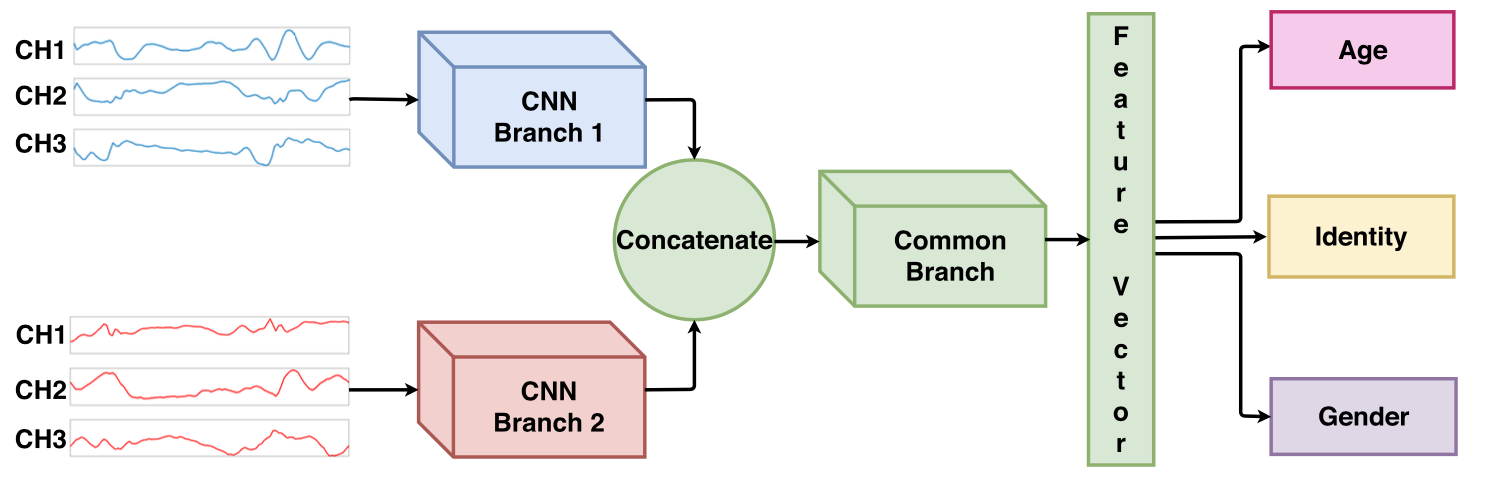
\includegraphics[width = 1 \linewidth]{images/paper5/architecture.png}
    \centering
    \caption{Pipeline for multi-task and multi-sensor learning in a gait-based system}
    \label{fig:pipeline}
\end{figure}

\subsubsection{Multi-task Approach}
The aim is to training a deep multi-task model (DTM). In order to do this, 
there must be a set of tuples $ I = (s_i, y_i^m, y_1^1, ..., y_i^T) $ where $ y_i^m $ is the label 
of the main task, $ y_i^t $, with $ t \in [1,T] $, is the label for each auxilary task. 
Each individual task has its own loss function \emph{L}. The loss function (\ref{loss-function}) is 
calculated on each sub-sequence \emph{s} and is formed by the product of each single 
loss function, of each task, with the weights ($ \lambda $)  associated at each task.
\begin{eqnarray}\label{loss-function}
    \emph{$ L_{DTM} (g(s,\theta), Y) $} & = & \lambda_{id}L_{id}(\hat{y}^{id}, y^{id}) \nonumber \\
                                        &   & + \lambda_{age}L_{age}(\hat{y}^{age}, y^{age}) \nonumber \\
                                        &   & + \lambda_{gender}L_{gender}(\hat{y}^{gender}, y^{gender}) 
\end{eqnarray}
Where $ Y = (y^{id}_i, y^{age}_i, y^{gender}_i) $ and $ L_{id}, L_{age}, L_{gender} $ are the loss functions of 
each tasks. As for the identity and gender tasks, their loss function is the 
cross-entropy and is calculated with the formula \ref{cross-entropy}.
\begin{equation}\label{cross-entropy}
    \emph{$ L_m(\hat{y}, c) $} = -\hat{y}_c+\log\sum^K_{k=1}e^{\hat{y}k} 
\end{equation}
Where $ \hat{y} $ is the ouput vector of the network, $ \hat{y}_c $ is the output for target class, 
$ \hat{y}_k $ is the \emph{k}-th component of the output vector, \emph{c} is the ground-truth class 
and \emph{K} is the total number of classes.

\subsubsection{Modality Fusion}
The merging of data that occurs at the input is useful for increasing the accuracy of the 
network and allows understanding the relationships between 
the different types of input data. Each data coming from a specific sensor 
will be inserted in an individual branch, composed of a specific number of 
convolutional layers that will calculate specific predictors for each sensor. 
In the end, the data will be concatenated in a common branch which has the 
task of extracting the combined features from all the sensors. Based on the accuracy metric, the 
layer that will return the best result will be selected.

\subsubsection{Identity Authentication}
An authentication process begins by submitting a sample of input to CNN. 
Within this, there may be a layer that will produce a vector of features. 
To find out which layer it is, a cross-validation process is performed. Once 
extracted, the features are normalized with the L2 standard. Subsequently 
a vector is calculated containing the Euclidean distances between the values 
given in input and those present in the training set. In order to calculate the 
\emph{Area Under Curve} (AUC) or the \emph{Equal-Error-Rate} (EER), these distances 
are transformed into probabilities.

\subsection{EXPERIMENTS AND RESULTS}
\subsubsection{Dataset}
The OU-ISIR dataset is composed in two parts. Part A contains data on 744 
individuals, each having two sub-sequence (s) recording at a rate of 100Hz 
via an IMU sensor located at the waist of each. The first sequence is used for 
training, the second for testing. The labels associated with each individual 
are: identity, gender and age (split in ranges). Part B, on the other hand, 
is composed of 495 individuals with 3 IMU sensors located on the body. For 
each individual and sensor, there are two sequences of walking levels, an up-slope 
walk sequence and the other down-slope walk. The data that will be 
merged are those coming from sensors such as accelerometer and gyroscope.
